\newpage
\section{k-Nearest Neighbours}
\label{sec:knn}

This section evaluates k-nearest neighbours as the first non-parametric and distance-based classifier in the project. Unlike logistic regression, which estimates a global vector of coefficients, k-nearest neighbours stores the training observations and classifies a new customer by comparing that customer with nearby training customers in the transformed feature space. The model is therefore useful as a contrast to the linear classifiers from Section~\ref{sec:linear-classification-and-logistic-regression}: logistic regression learns global feature weights, whereas k-nearest neighbours relies directly on local similarity.

The same validation discipline is used as in the previous modelling sections. The held-out test set is not used. All reported results are based on stratified cross-validation inside the training set. Preprocessing is kept inside the scikit-learn pipeline so that standardization and one-hot encoding are fitted only on each fold's training data.

The results in this section should be interpreted as a development-stage comparison of kNN configurations. The selected kNN model is the strongest configuration in the tried grid according to the chosen selection criterion. It is not a final statistical claim that this exact value of \(k\), distance metric, and weighting rule is uniquely optimal in the population.

\subsection{k-nearest-neighbour prediction rule}

Let the training set be
\[
\mathcal{D}_{\mathrm{train}}
=
\{(x_i,y_i)\}_{i=1}^{n},
\]
where \(x_i \in \mathbb{R}^{p}\) is the transformed feature vector for customer \(i\), and \(y_i \in \{0,1\}\) is the binary churn label. For a new customer with feature vector \(x\), k-nearest neighbours first finds the \(k\) training observations closest to \(x\) according to a chosen distance function. Let this neighbour set be denoted by
\[
\mathcal{N}_k(x).
\]
For unweighted binary classification, the estimated churn probability is the fraction of neighbours that churned:
\[
\widehat{p}(Y=1 \mid X=x)
=
\frac{1}{k}
\sum_{i \in \mathcal{N}_k(x)} y_i.
\]
The default hard classification rule at threshold \(0.5\) is
\[
\widehat{y}
=
\mathbb{1}
\left\{
\widehat{p}(Y=1 \mid X=x) \geq 0.5
\right\}.
\]
Thus, the model predicts churn when churners form at least half of the local neighbourhood.

A distance-weighted variant gives closer neighbours more influence:
\[
\widehat{p}(Y=1 \mid X=x)
=
\frac{
\sum_{i \in \mathcal{N}_k(x)} w_i(x)y_i
}{
\sum_{i \in \mathcal{N}_k(x)} w_i(x)
}.
\]
In this section, both uniform and distance-based voting are evaluated.

\subsection{Distance, scaling, and one-hot encoded features}

The distance definition is central to k-nearest neighbours. Two common distances are the Manhattan distance,
\[
d_1(x,x')
=
\sum_{j=1}^{p}
|x_j-x'_j|,
\]
and the Euclidean distance,
\[
d_2(x,x')
=
\sqrt{
\sum_{j=1}^{p}
(x_j-x'_j)^2
}.
\]
Both are special cases of the Minkowski distance. In the implementation, Manhattan distance corresponds to \(p=1\), while Euclidean distance corresponds to \(p=2\).

Because k-nearest neighbours computes distances directly from feature values, scaling is essential. Without standardization, variables with larger numeric ranges can dominate the distance calculation. For example, \texttt{TotalCharges} has a much larger raw range than \texttt{tenure} or \texttt{MonthlyCharges}. Therefore, numeric variables are standardized inside the preprocessing pipeline. Categorical variables are one-hot encoded, which allows k-nearest neighbours to operate on mixed tabular data, but also changes the geometry of the feature space. After one-hot encoding, similarity is measured in a higher-dimensional indicator space, which may not always correspond to intuitive customer similarity.

\subsection{The role of \(k\)}

The number of neighbours \(k\) controls the smoothness of the classifier. Small values of \(k\) produce highly local predictions. For example, when \(k=1\), the prediction copies the label of the single nearest training observation. This can produce low-bias but high-variance decision boundaries that are sensitive to noise.

Larger values of \(k\) average over more training observations. This usually increases bias but reduces variance, producing smoother and more stable predictions. If \(k\) becomes too large, however, predictions approach the global class distribution and the model can underfit. Therefore, \(k\) is a true model-complexity hyperparameter and must be selected using validation data rather than the held-out test set.

\subsection{Hyperparameter grid}

The k-nearest-neighbour experiment uses a transparent cross-validated grid search. The grid varies the number of neighbours, the voting scheme, and the distance metric:
\[
k \in \{1,3,5,7,11,15,21,31,51,75,101\},
\]
\[
\texttt{weights} \in \{\texttt{uniform},\texttt{distance}\},
\]
\[
p \in \{1,2\}.
\]
The \(p=1\) setting corresponds to Manhattan distance, and \(p=2\) corresponds to Euclidean distance. The selection rule chooses the configuration with the highest cross-validated PR-AUC, using balanced accuracy and F1 as secondary criteria if needed. PR-AUC is used as the primary criterion because churn is the minority class, and the positive-class ranking quality is important.

Because this grid tries multiple configurations, the winning cross-validated score should be interpreted with the model-selection caveat from Section~\ref{sec:statistical-evaluation-methodology}. It identifies a strong configuration within the tried grid, but the observed best score can contain some selection optimism.

\subsection{Grid-search behaviour}

Figure~\ref{fig:knn-pr-auc-by-k} shows the cross-validated PR-AUC across the neighbour grid. Performance improves strongly as \(k\) increases from very small values. This pattern indicates that small neighbourhoods are too noisy for this dataset. Larger neighbourhoods smooth over local irregularities and give more stable churn rankings.

\begin{figure}[H]
\centering
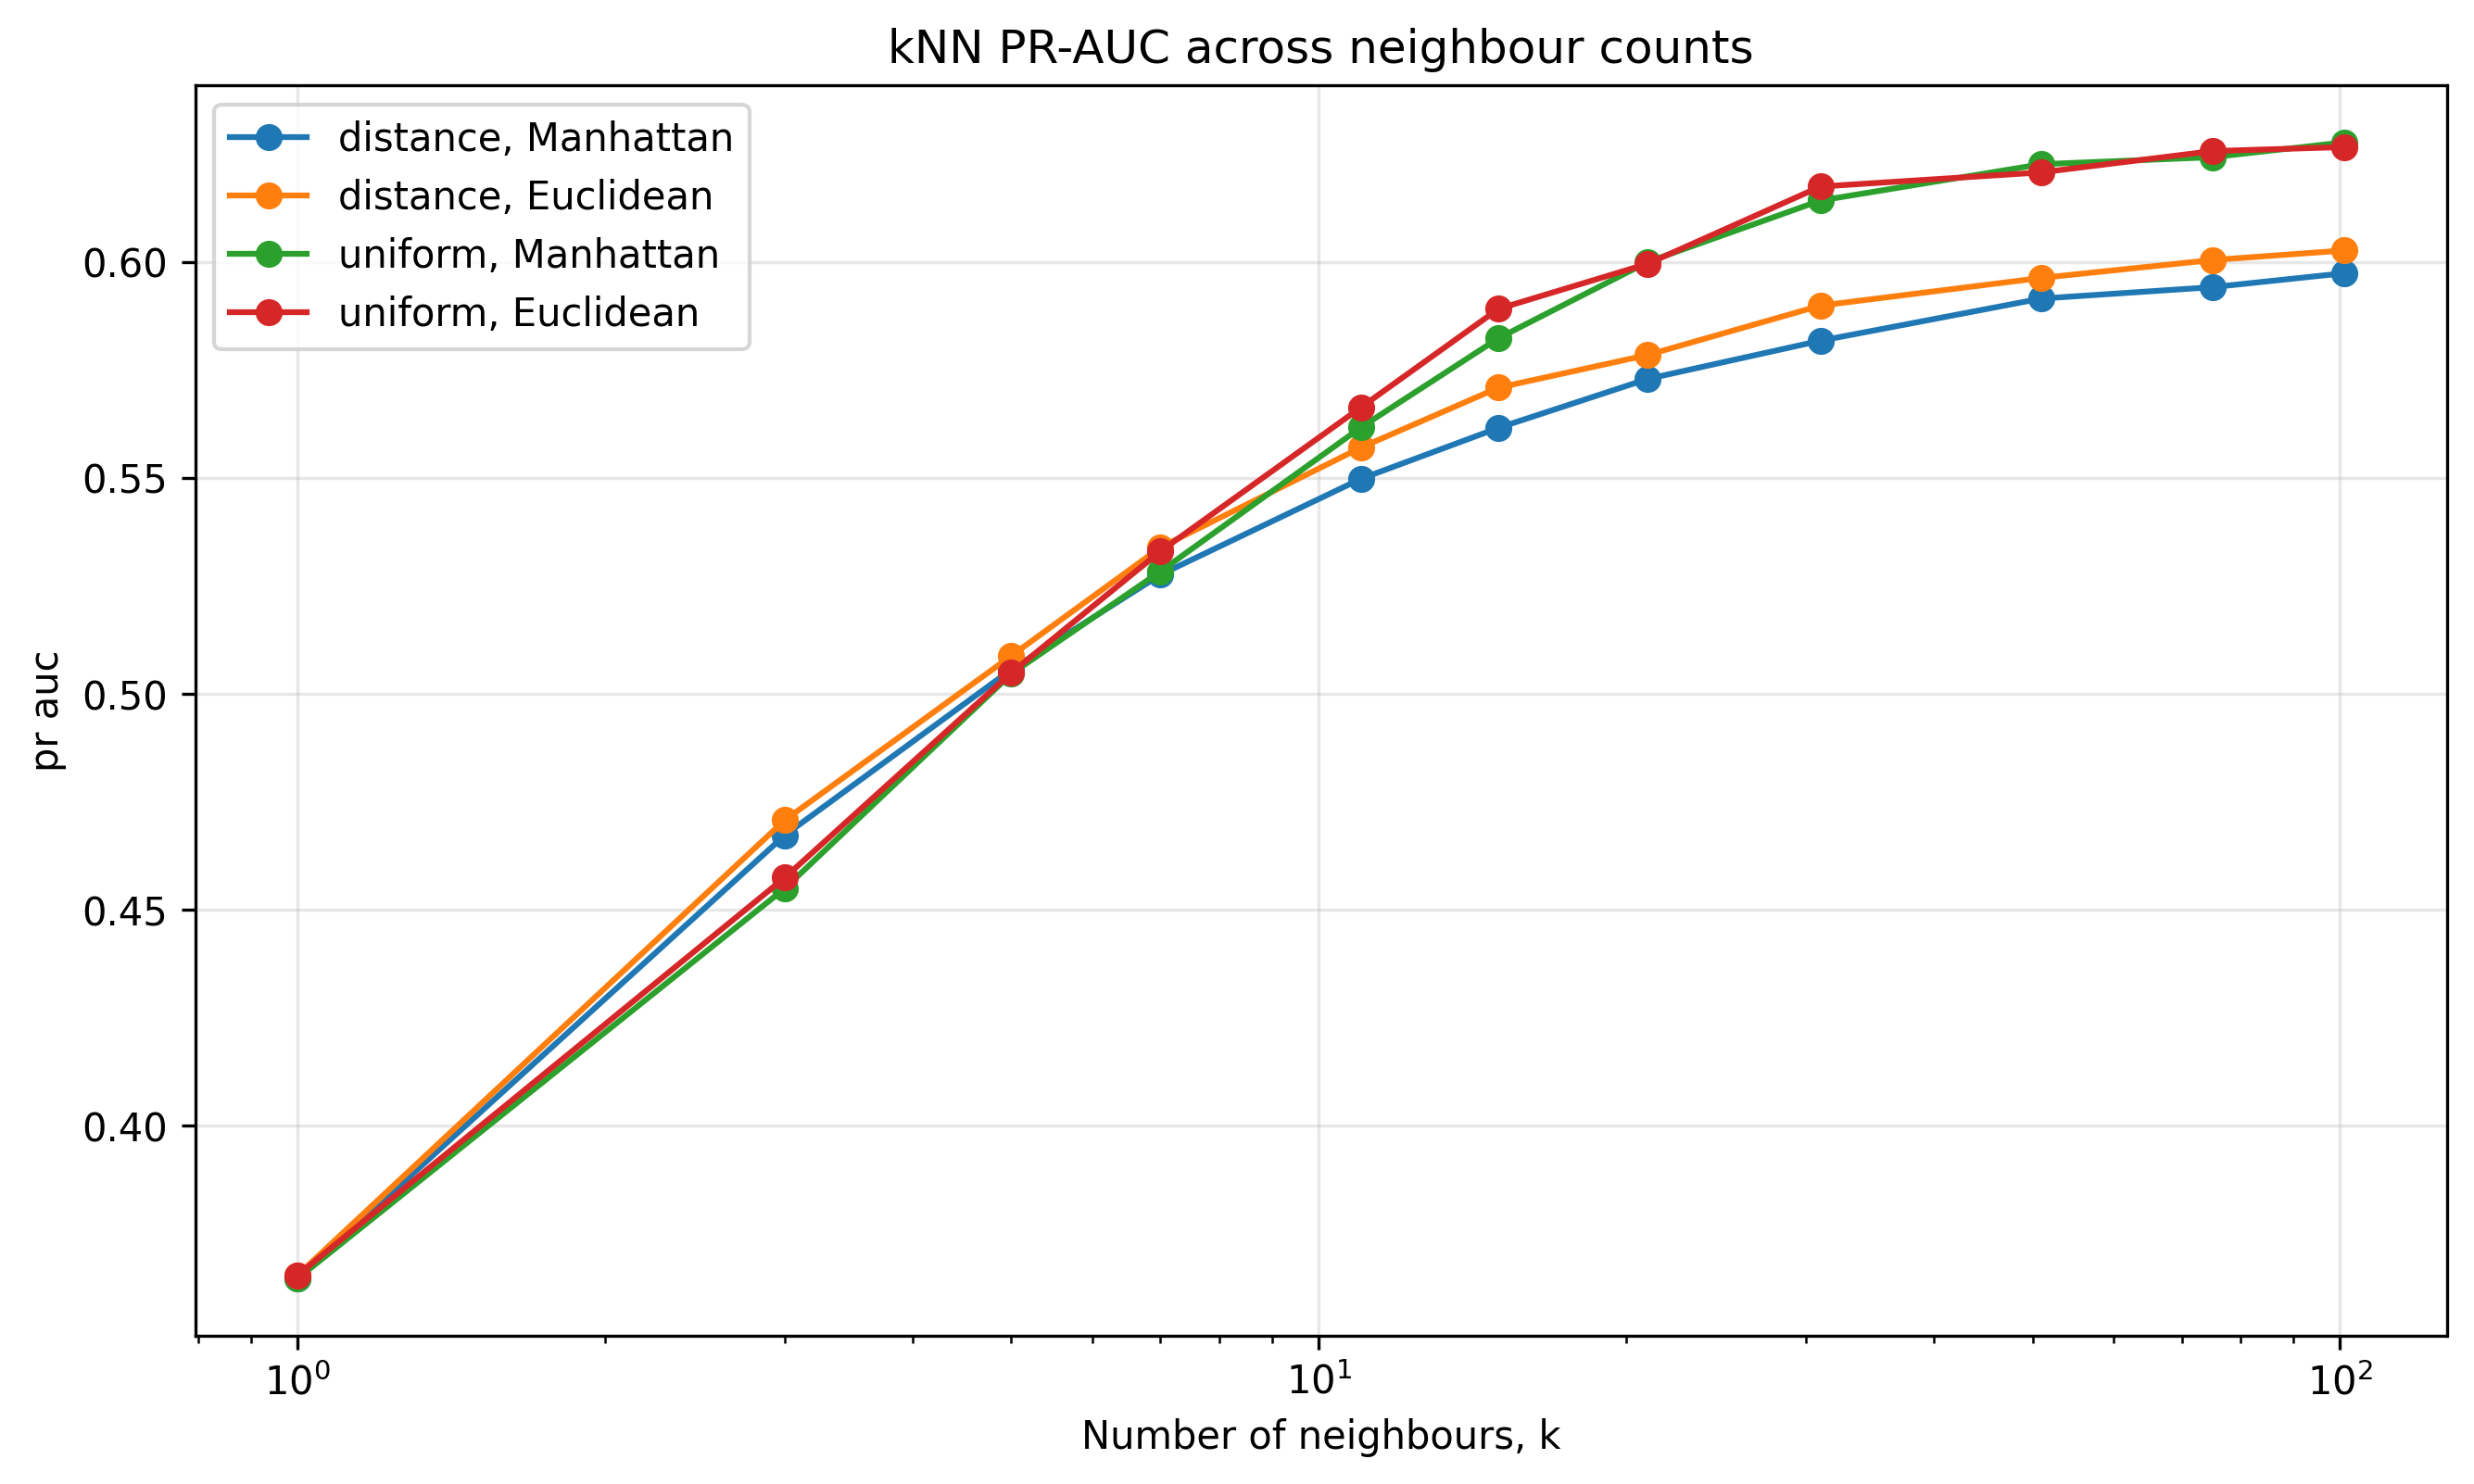
\includegraphics[width=0.88\textwidth]{../figures/knn_pr_auc_by_k.png}
\caption{kNN PR-AUC across neighbour counts}
\label{fig:knn-pr-auc-by-k}
\end{figure}

Figure~\ref{fig:knn-balanced-accuracy-by-k} shows the same grid from the perspective of balanced accuracy. Balanced accuracy also improves as \(k\) increases, but it peaks somewhat earlier than PR-AUC for some configurations. This difference is expected because PR-AUC evaluates ranking quality across thresholds, while balanced accuracy depends on the default hard classification threshold.

\begin{figure}[H]
\centering
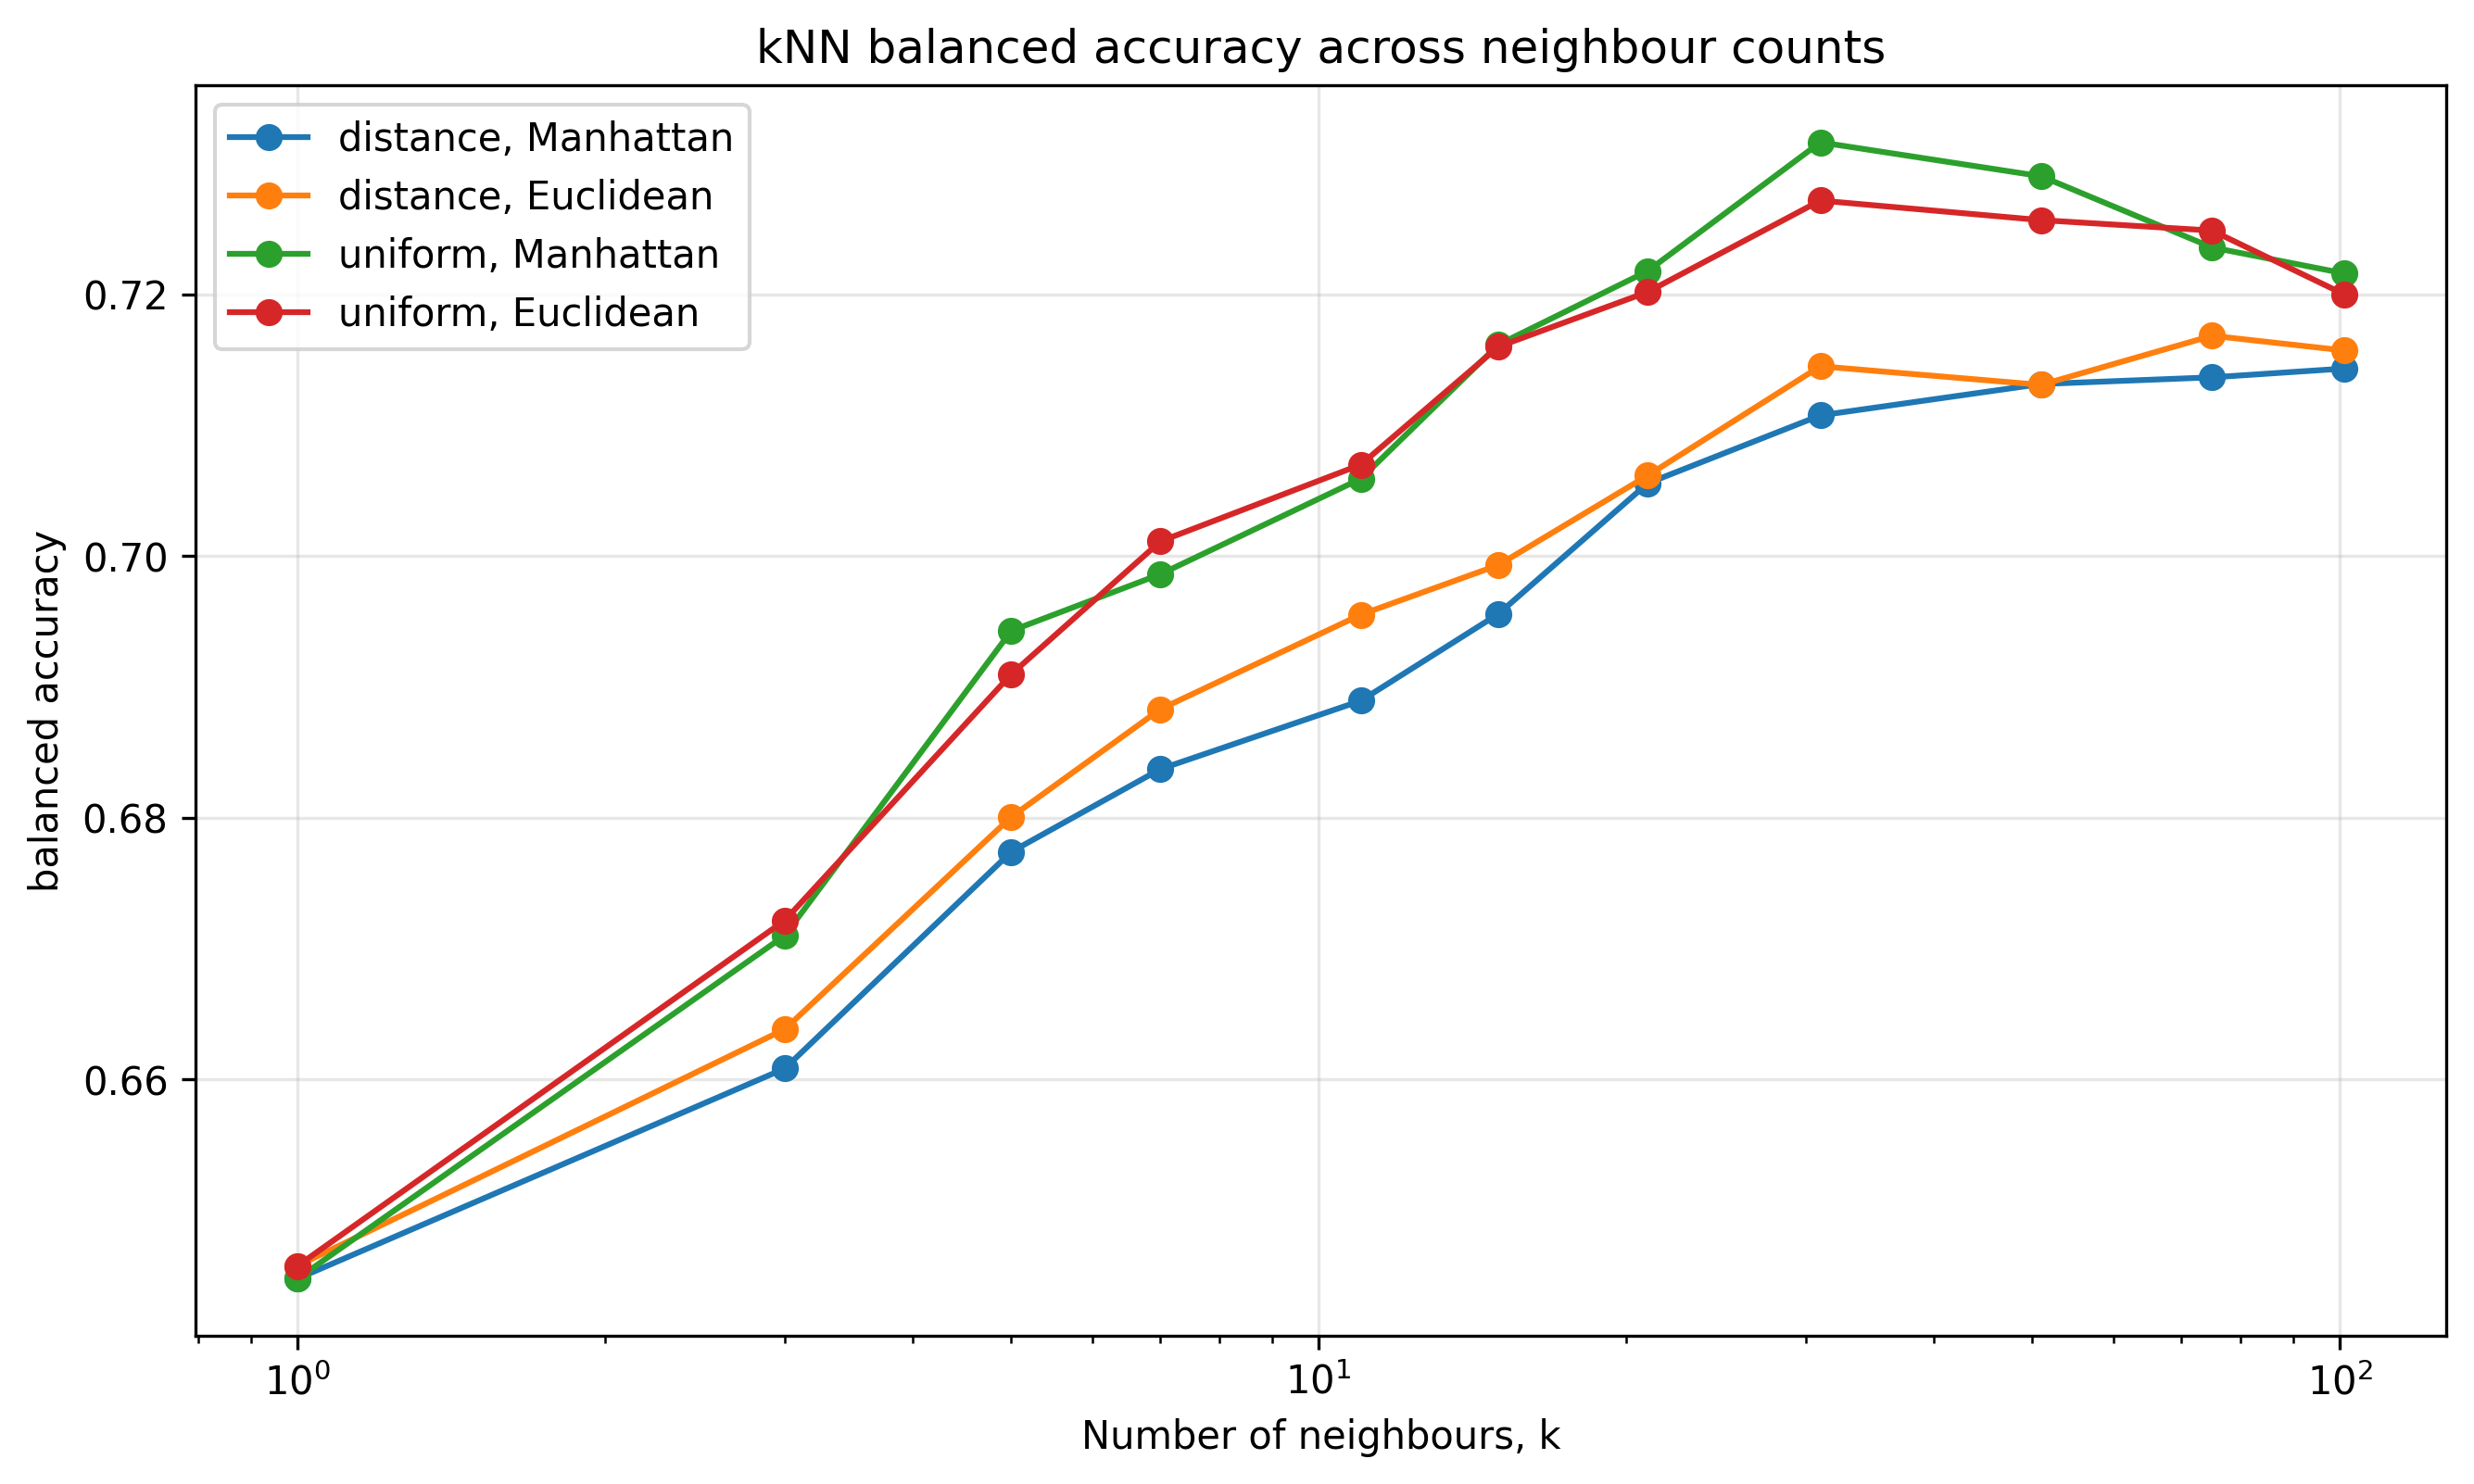
\includegraphics[width=0.88\textwidth]{../figures/knn_balanced_accuracy_by_k.png}
\caption{kNN balanced accuracy across neighbour counts}
\label{fig:knn-balanced-accuracy-by-k}
\end{figure}

The strongest configuration by PR-AUC in the tried grid is the uniform-weighted Manhattan model with \(k=101\). Uniform weighting outperforms distance weighting among the best configurations. This suggests that allowing very close neighbours to dominate does not improve development-stage generalization in this transformed feature space. A smoother average over many neighbours is more stable.

The interpretation should focus on the broader pattern rather than the exact integer \(k=101\). The grid evidence suggests that very small neighbourhoods are too noisy and that larger, smoother neighbourhoods work better for this representation. It does not prove that \(k=101\) is uniquely optimal; nearby large-\(k\) settings may be practically similar.

\subsection{Model comparison}

Table~\ref{tab:knn-model-comparison} compares the default \(k=5\) Euclidean kNN model with the selected kNN model. The selected model improves substantially over the default setting. Accuracy rises from approximately \(0.765\) to \(0.792\), balanced accuracy from approximately \(0.691\) to \(0.722\), ROC-AUC from approximately \(0.782\) to \(0.836\), and PR-AUC from approximately \(0.505\) to \(0.628\). This difference is large enough to support the development-stage conclusion that tuning \(k\), distance, and weighting is important for kNN on this dataset.

\begin{table}[H]
\centering
\small
\begin{tabular}{lrrrrrrrr}
\toprule
Model & Accuracy & Bal. Acc. & Precision & Recall & Specificity & F1 & ROC-AUC & PR-AUC \\
\midrule
Selected kNN, \(k=101\), uniform, Manhattan
& 0.792 & 0.722 & 0.617 & 0.571 & 0.872 & 0.593 & 0.836 & 0.628 \\
kNN, \(k=5\), uniform, Euclidean
& 0.765 & 0.691 & 0.561 & 0.532 & 0.849 & 0.546 & 0.782 & 0.505 \\
\bottomrule
\end{tabular}
\caption{kNN model comparison using cross-validated out-of-fold predictions}
\label{tab:knn-model-comparison}
\end{table}

The corresponding positive-first confusion-matrix counts are shown in Table~\ref{tab:knn-confusion}. The selected model detects more churners and also produces fewer false positives than the default \(k=5\) model. Specifically, the selected model gives \(854\) true positives and \(530\) false positives, compared with \(796\) true positives and \(623\) false positives for the default model.

\begin{table}[H]
\centering
\small
\begin{tabular}{lrrrr}
\toprule
Model & TP & FN & FP & TN \\
\midrule
Selected kNN, \(k=101\), uniform, Manhattan & 854 & 641 & 530 & 3609 \\
kNN, \(k=5\), uniform, Euclidean & 796 & 699 & 623 & 3516 \\
\bottomrule
\end{tabular}
\caption{Positive-first confusion-matrix counts for kNN models}
\label{tab:knn-confusion}
\end{table}

Compared with logistic regression from Section~\ref{sec:linear-classification-and-logistic-regression}, selected kNN has lower development-stage ranking metrics. The selected logistic regression model had ROC-AUC around \(0.846\) and PR-AUC around \(0.658\), while selected kNN has ROC-AUC around \(0.836\) and PR-AUC around \(0.628\). This suggests that the global feature-weighting structure learned by logistic regression is more effective than direct distance-based local similarity for this transformed Telco churn dataset.

This comparison should still be read as development-stage evidence. The gap is meaningful enough to keep logistic regression as the stronger candidate so far, but final statistical claims about model-family superiority are deferred to the later model-comparison and test-evaluation stages.

\subsection{Threshold behaviour}

The selected kNN model provides predicted probabilities from neighbour proportions. Figure~\ref{fig:knn-threshold-tradeoff} shows how precision, recall, specificity, and F1 change as the classification threshold varies. Lower thresholds identify many more churners but also flag many more non-churners. Higher thresholds improve precision and specificity but miss more churners.

\begin{figure}[H]
\centering
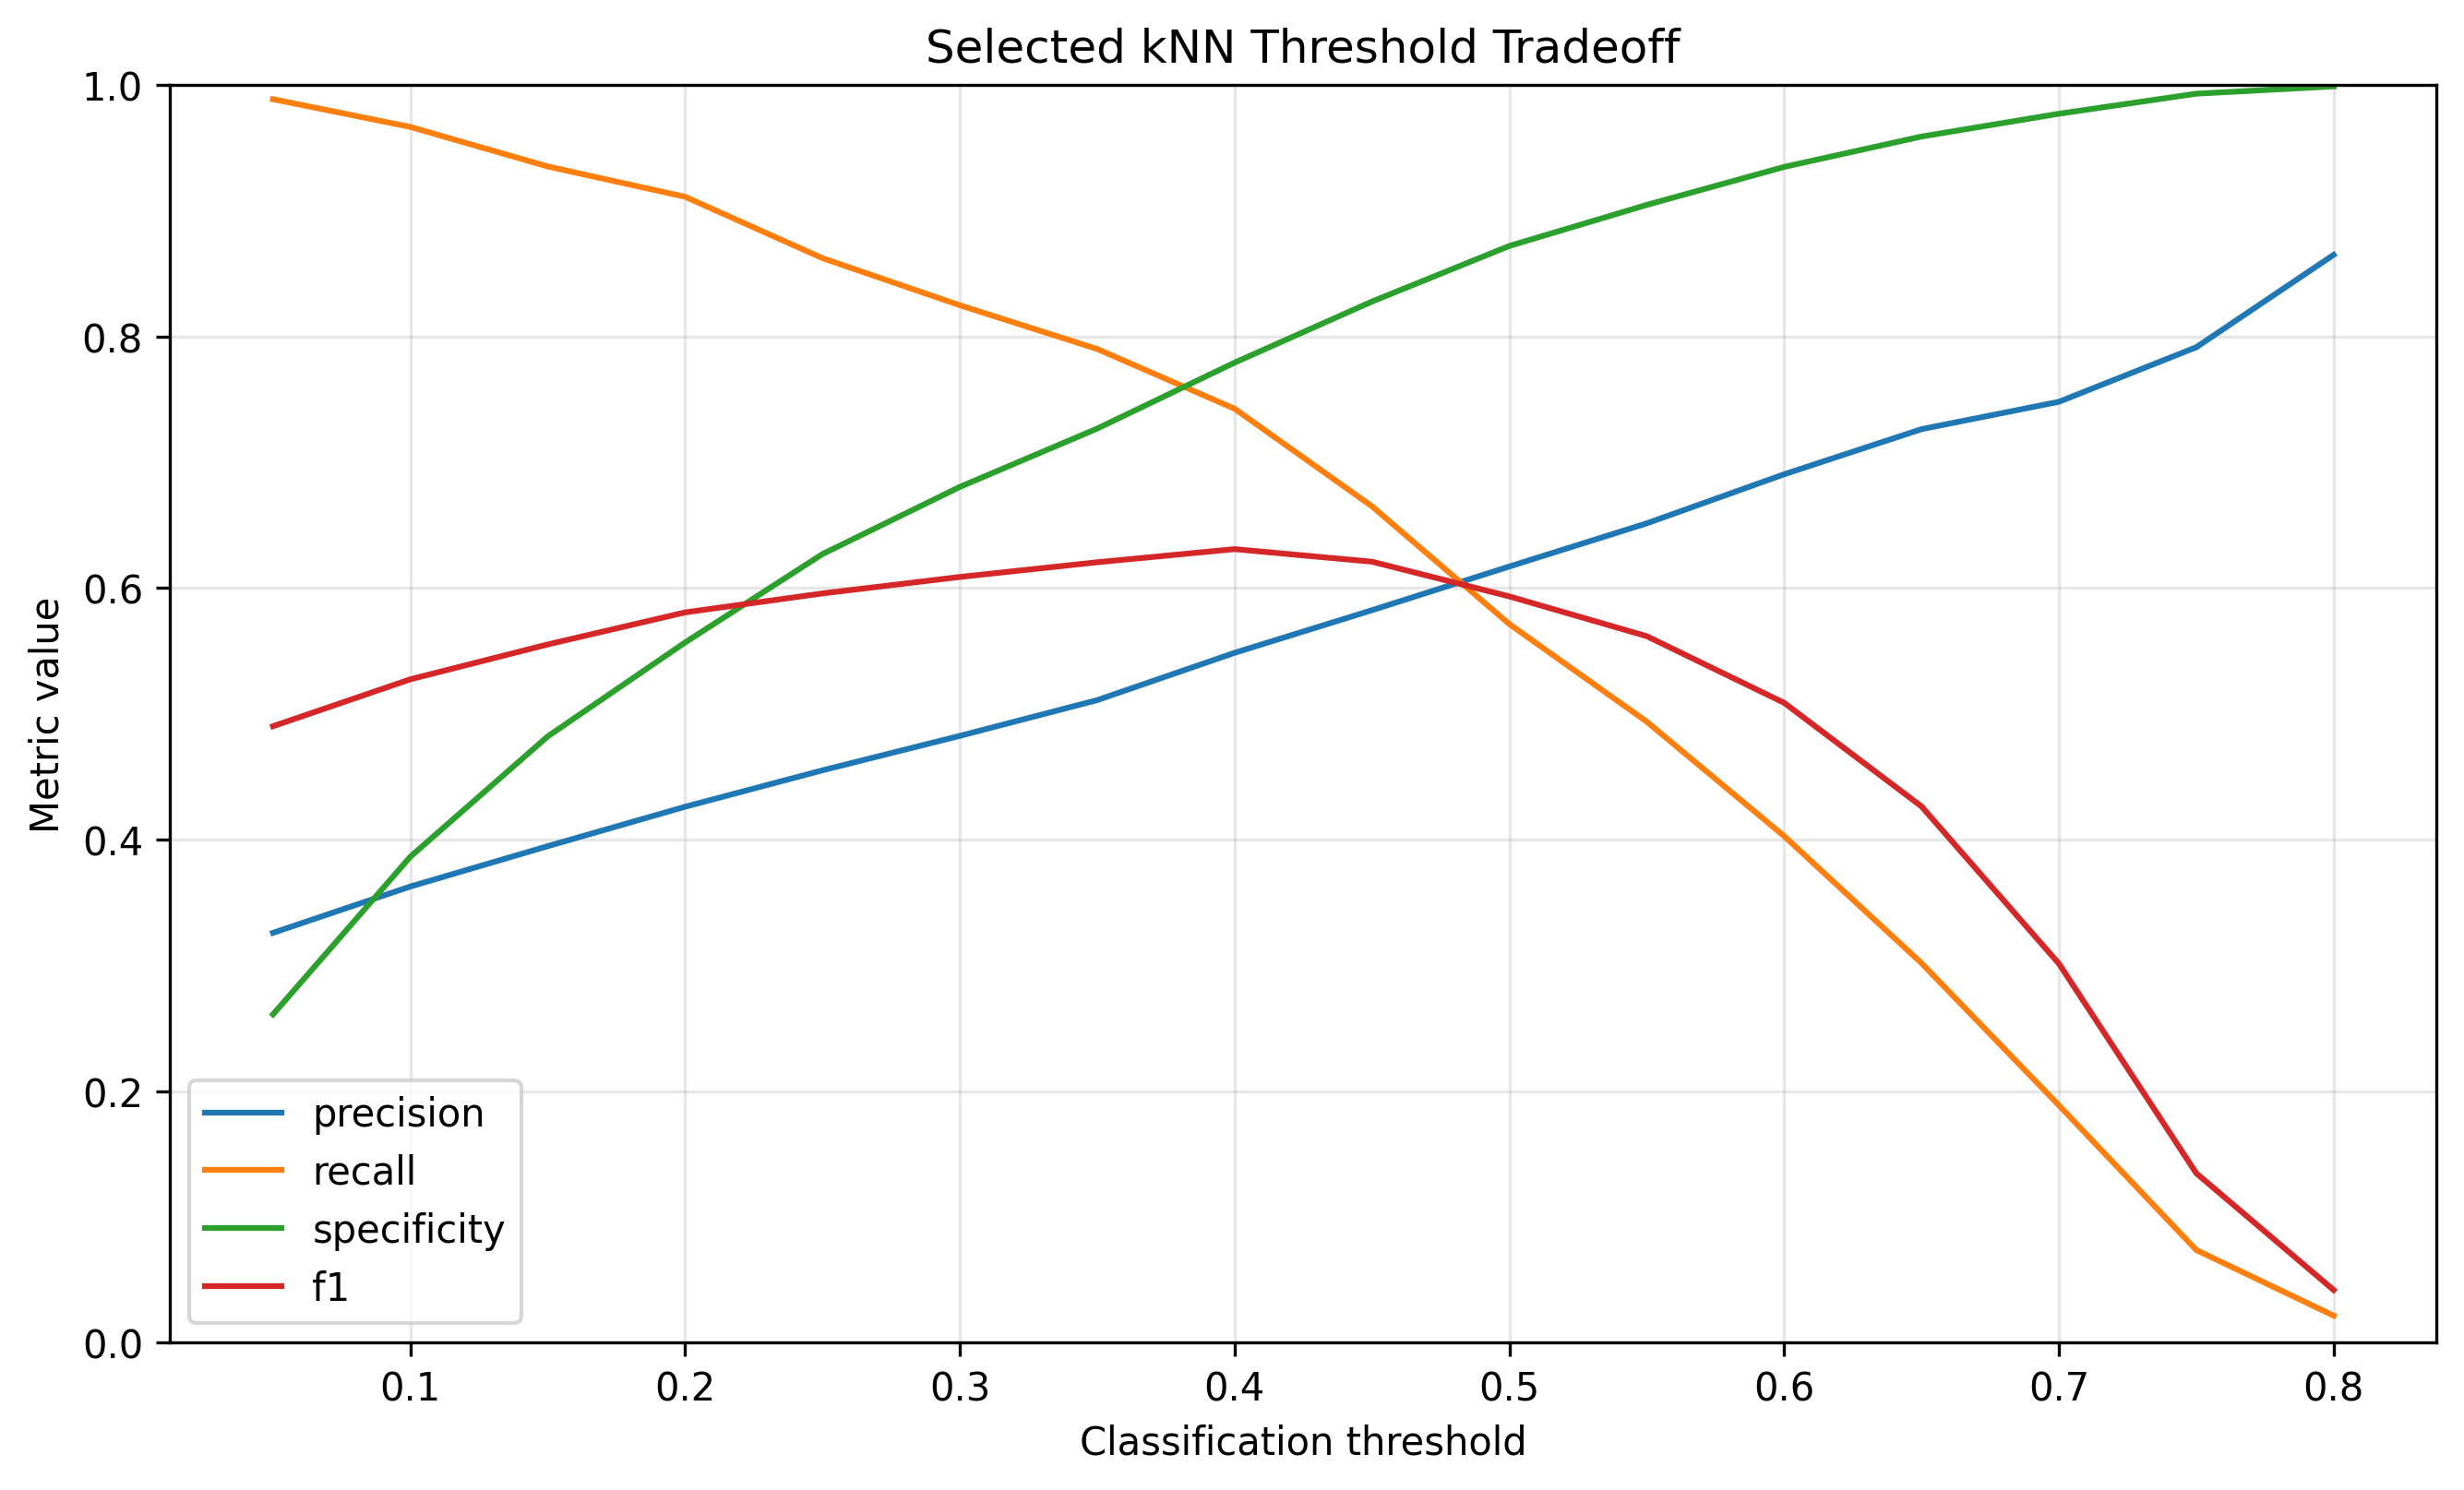
\includegraphics[width=0.88\textwidth]{../figures/knn_threshold_tradeoff.png}
\caption{Threshold tradeoff for the selected kNN model}
\label{fig:knn-threshold-tradeoff}
\end{figure}

At threshold \(0.25\), recall is approximately \(0.862\), but precision is only approximately \(0.455\). At threshold \(0.40\), the model reaches a more balanced operating point, with precision approximately \(0.548\), recall approximately \(0.742\), specificity approximately \(0.779\), and F1 approximately \(0.631\). At the default threshold \(0.50\), precision improves to approximately \(0.617\), but recall falls to approximately \(0.571\). This again shows that threshold \(0.50\) is not necessarily the best operating point for churn detection.

These threshold results are diagnostic rather than final. Threshold selection is itself a modelling decision and is postponed until the later model-comparison stage, where the project objective and candidate model families can be considered together.

\subsection{ROC and precision-recall curves}

Figure~\ref{fig:knn-roc-curve} shows the ROC curve for the selected kNN model. The ROC-AUC is approximately \(0.836\), clearly above the random-ranking line. This indicates that the selected kNN model ranks churners above non-churners much better than chance.

\begin{figure}[H]
\centering
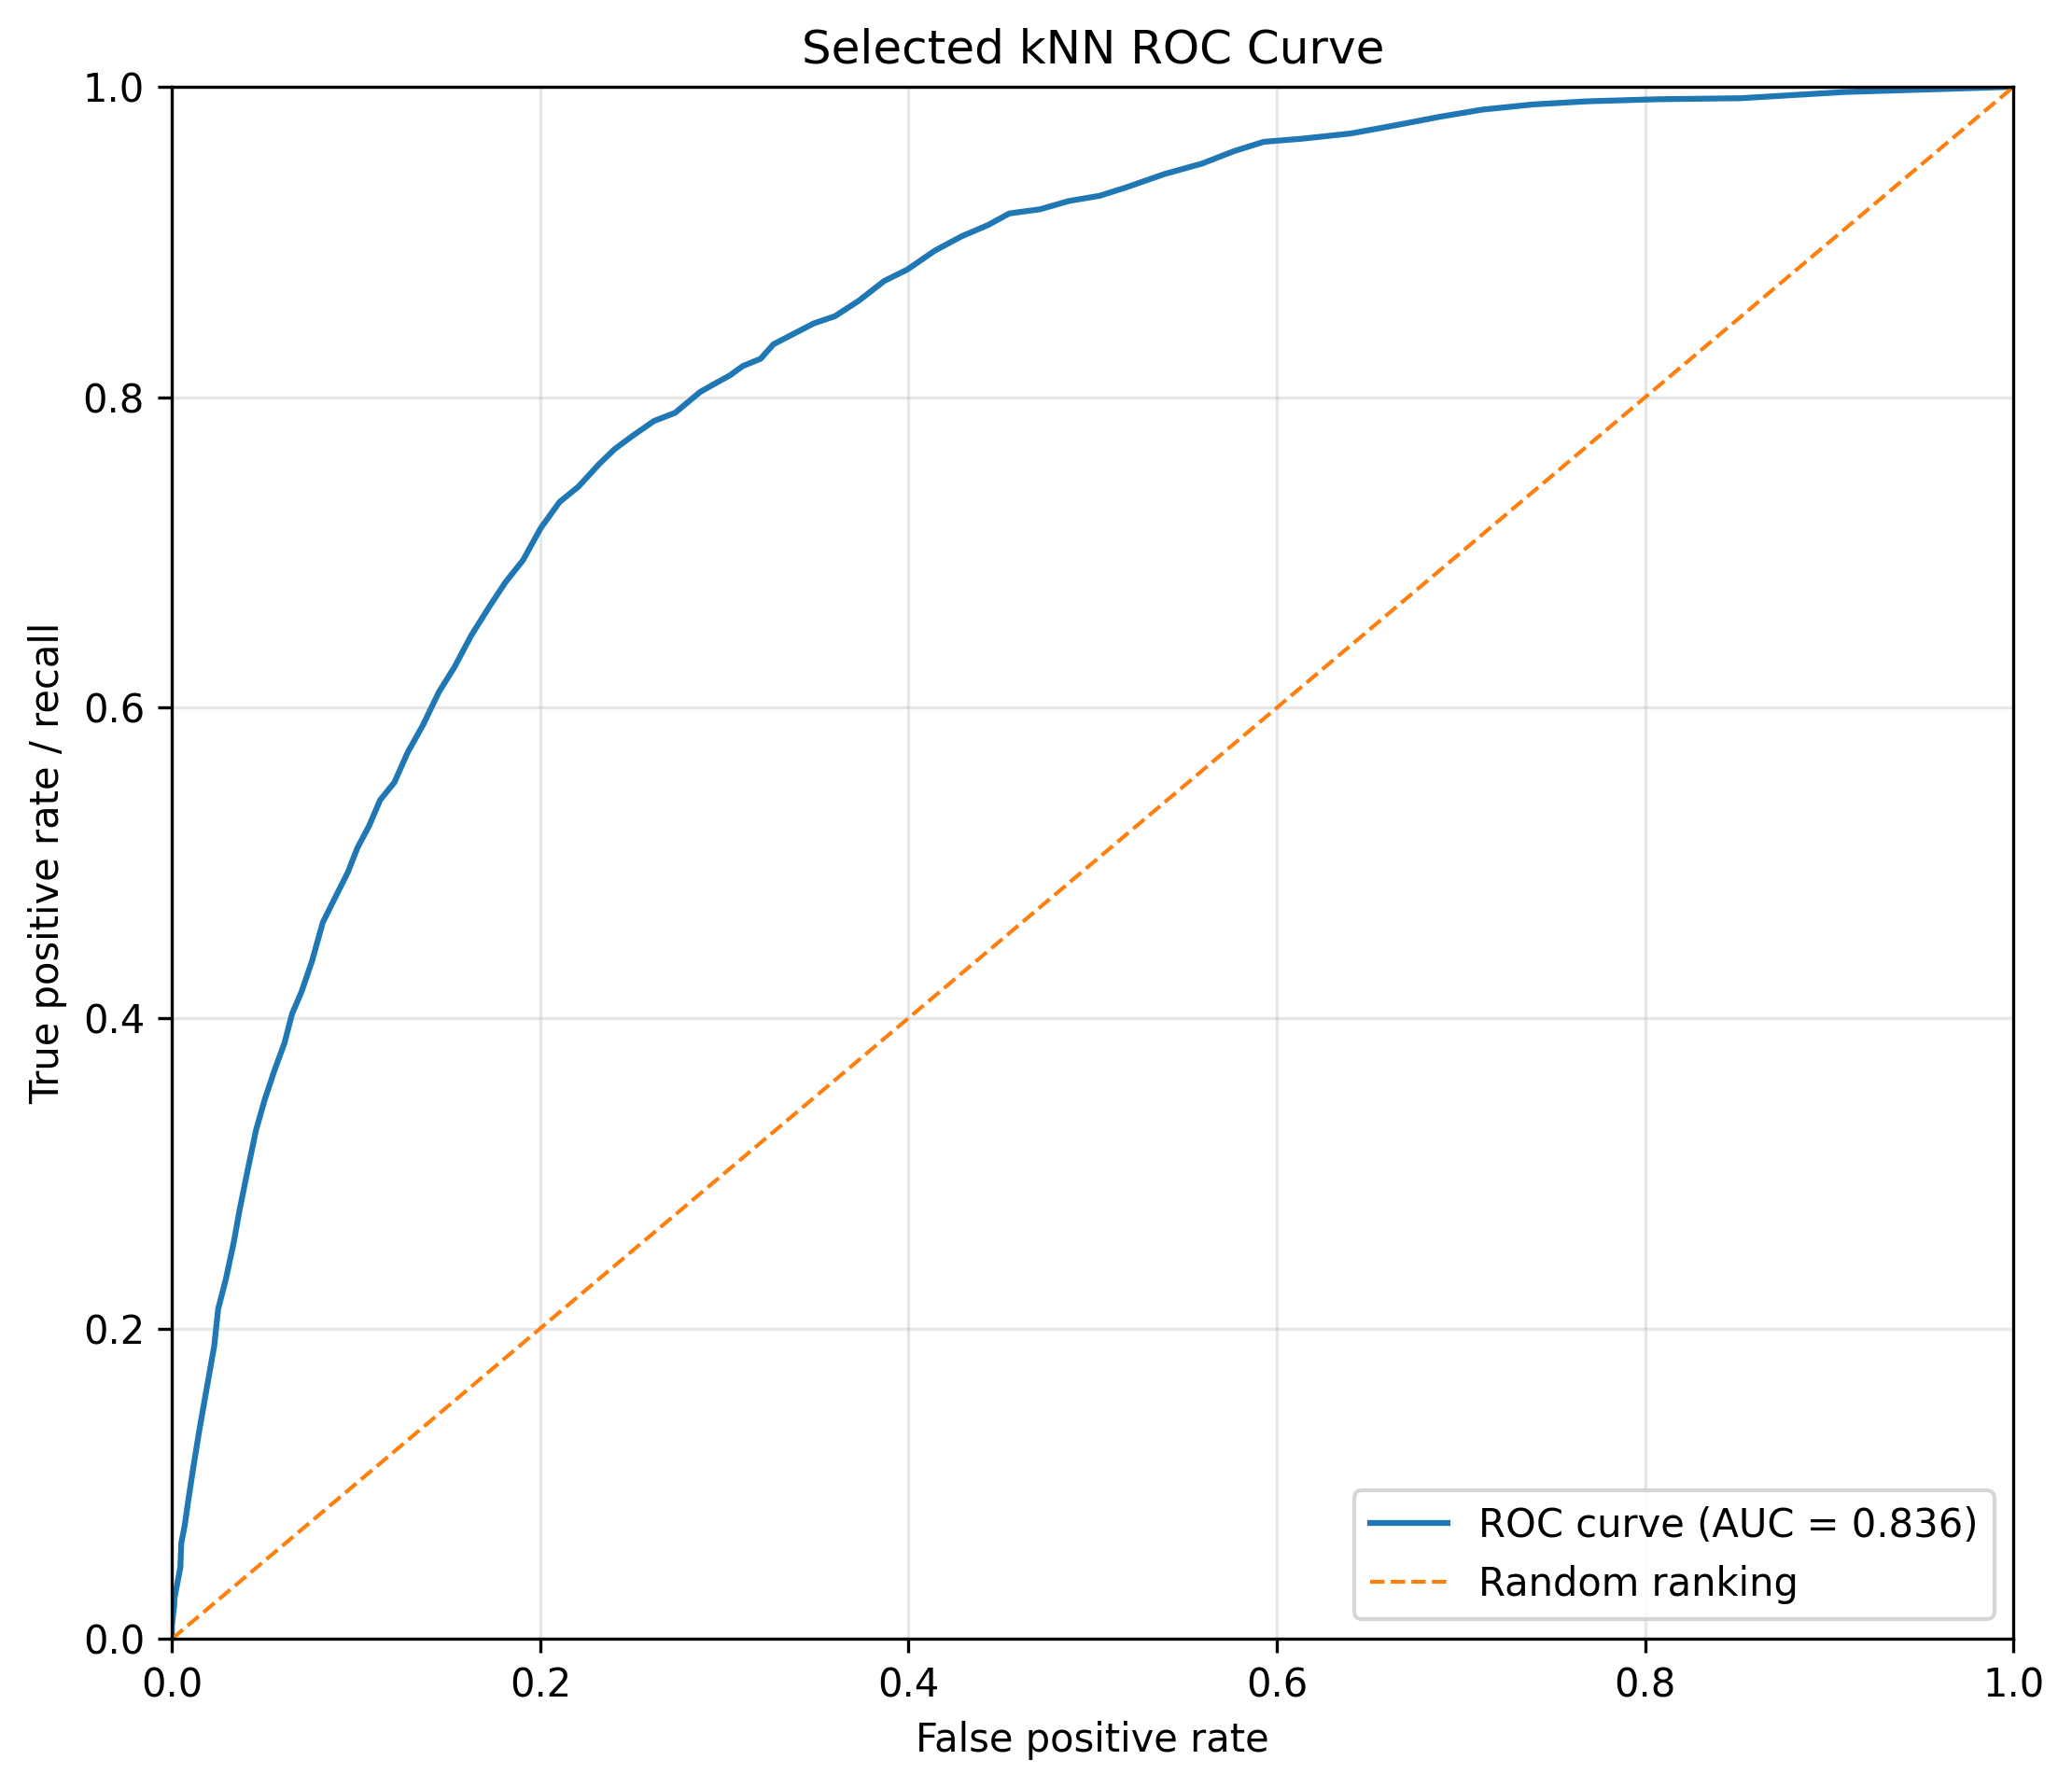
\includegraphics[width=0.72\textwidth]{../figures/knn_roc_curve.png}
\caption{ROC curve for the selected kNN model}
\label{fig:knn-roc-curve}
\end{figure}

Figure~\ref{fig:knn-pr-curve} shows the precision-recall curve. The PR-AUC is approximately \(0.631\), well above the positive-rate baseline of approximately \(0.265\). This confirms that kNN has useful positive-class retrieval ability. However, it remains below the logistic regression PR-AUC from Section~\ref{sec:linear-classification-and-logistic-regression}. The gap is not extremely large, so it should be interpreted as development-stage evidence rather than final statistical proof.

\begin{figure}[H]
\centering
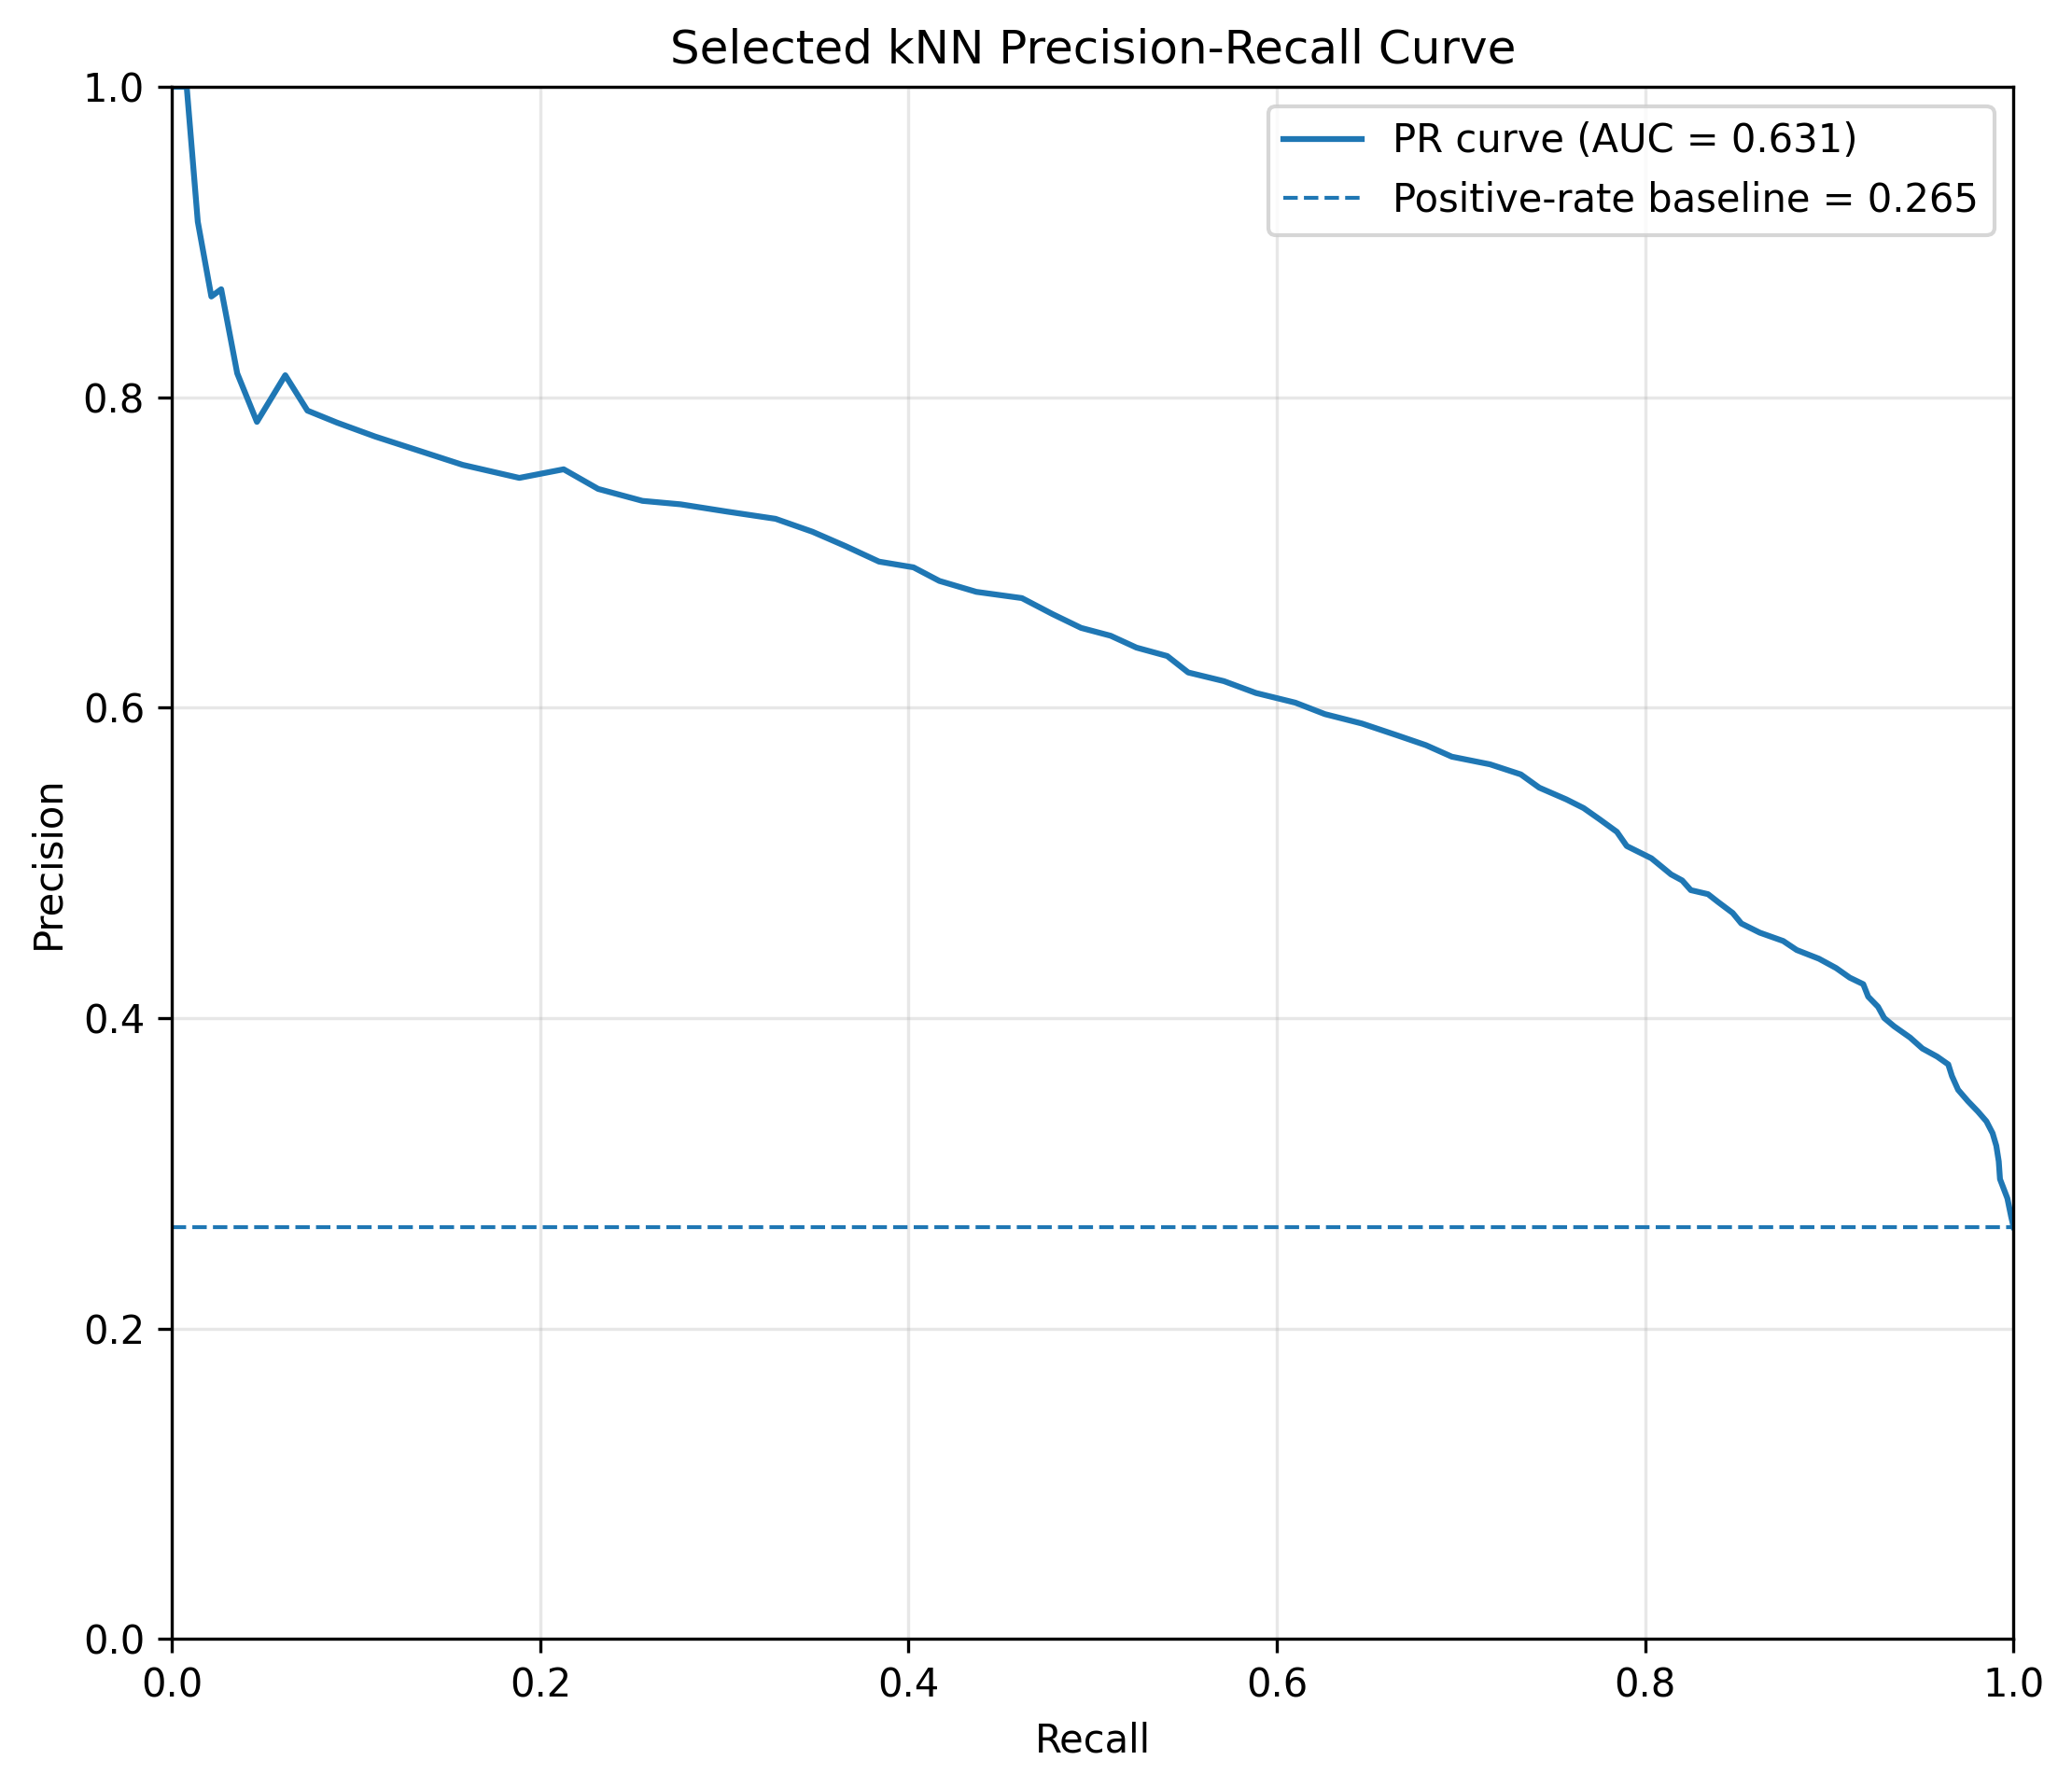
\includegraphics[width=0.72\textwidth]{../figures/knn_precision_recall_curve.png}
\caption{Precision-recall curve for the selected kNN model}
\label{fig:knn-pr-curve}
\end{figure}

\subsection{Summary}

The k-nearest-neighbour experiment shows that distance-based classification learns meaningful churn structure, but it does not outperform logistic regression in the current development-stage comparison. The most important findings are as follows. First, kNN performance is highly sensitive to the number of neighbours. Small \(k\) values are too noisy, while larger neighbourhoods perform better. Second, uniform weighting works better than distance weighting in the strongest configurations. Third, the strongest PR-AUC in the grid is obtained by the uniform Manhattan model with \(k=101\), which is a relatively smooth kNN classifier. Fourth, the selected kNN model improves substantially over the default \(k=5\) baseline, but remains below logistic regression in ROC-AUC and PR-AUC.

The section is useful because it introduces local, distance-based learning and the bias-variance role of \(k\). It also illustrates a limitation of distance-based methods on one-hot encoded tabular data: the constructed distance space may not be as informative as a model that learns feature weights directly. The exact selected \(k\) should not be overinterpreted; the robust lesson is that smoothing over a larger neighbourhood is preferable to very local neighbour voting for this feature representation. The next modelling stage introduces Naive Bayes before the project moves to tree-based models.
